El módulo del cliente se compone de varios paquetes esenciales, cada uno con un rol específico en la estructura del sistema:
\begin{itemize}
	\item \textbf{Componentes:}  Este paquete contiene todos los componentes de la interfaz de usuario que se componen para formar las diferentes vistas de la aplicación.
	\item \textbf{Layouts:} Define la estructura general de las páginas, utilizando componentes y temas para asegurar una apariencia consistente en toda la aplicación.
	\item \textbf{Tema:} Se utiliza para aplicar estilos y temas consistentes a los componentes y layouts, asegurando una experiencia de usuario uniforme.
	\item \textbf{Hooks:} Almacena la lógica reutilizable que puede ser compartida entre diferentes componentes. Utiliza APIs y contextos para manejar datos y estados.
	\item \textbf{APIs:} Gestiona la comunicación con el servidor, realizando llamadas a las diferentes APIs necesarias para la funcionalidad de la aplicación.
	\item \textbf{Contextos:} Proporciona un mecanismo para compartir estados y datos entre componentes sin necesidad de pasar props manualmente en cada nivel.
\end{itemize}
El diagrama también muestra cómo el cliente se comunica con el servidor, asegurando que los datos fluyan correctamente entre el frontend y el backend.

\begin{figure}[H]
	\centering
	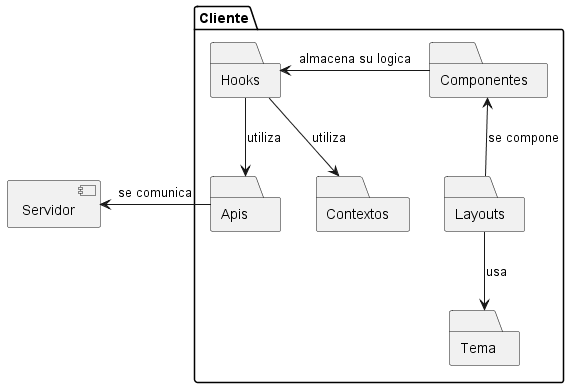
\includegraphics[width=1\linewidth]{6-DiseñoDelSistemaDeInformacion/Modulos/cliente.png}
	\caption{Diagrama de paquetes del Cliente}
\end{figure}